\documentclass[letterpaper, 10 pt]{report}

% For handling graphics
\usepackage{graphicx}
% For colors
\usepackage{color}
% For hyperlink
\usepackage{hyperref}
\hypersetup{
    colorlinks,
    linktoc=all,
    citecolor=black,
    filecolor=black,
    linkcolor=black,
    urlcolor=blue
}
% For mathematics
\usepackage{mathtools}
\usepackage[margin=1.0in]{geometry}

% -------------------------------------------------------------------------------------
% TITLE PAGE
% -------------------------------------------------------------------------------------
\begin{document}
\begin{titlepage}
\center
% Headings
\textsc{\LARGE Georgia Institute of Technology}\\[1.5cm]
\textsc{\large Center for Robotics \& Intelligent Machines}\\[0.5cm]
\textsc{\large Humanoid Robotics Lab}\\[0.5cm]
% Title
\rule{\linewidth}{0.5mm}\\[0.4cm]
{\huge \bfseries Hubo Notebook}\\[0.4cm]
\rule{\linewidth}{0.5mm}\\[1.5cm]
% Author
\textsc{\normalsize Peter Vieira}\\[1.5cm]
% Image
\includegraphics[width=5.0cm]{resources/hubo-titlepage}
% Fill rest of page with whitespace
\vfill
\end{titlepage}

% -------------------------------------------------------------------------------------
% JOURNAL ENTRIES
% -------------------------------------------------------------------------------------
\section*{ICRA Submission Critical Tasks}
Pete
\begin{itemize}
  \item Fix Biped walking.
  \begin{itemize}
    \item Test landing controller using impedance controller.
    \item Try implementing Youngbum's ZMP Tracking controller.
  \end{itemize}
\end{itemize}
Grey
\begin{itemize}
  \item Fix waist control.
  \item Goto last command in Rviz.
  \item Add end-effector 6-DOF interactive marker.
  \item Add other Rviz feature requests.
\end{itemize}

\section*{Tasks}
\begin{itemize}
\item Merge hubo-motion-rt master branch into the devel/biped-quad branch and use control-daemon's trajectory mode.
\item Change max number of steps in hubo\_walk.
\item Add balance-cmd channel check in iterative function in zmpwalkgenerator, like comIK and addFootstep.
\item Make it so we can walk while keeping arms in their current positions for carrying objects.
\item Modify the impedance controller logic to act as a landing controller during single-support phase.
\item Test and fix biped walking on the robot.
\item Get walking to a point/theta written and working.
\item Add state feedback from Walker.
\item Clone Matt's logger and add stance to it.
\item \textbf{DONE 9/5} Verify and test impedance controller. \newline
\textbf{Result} Sort of worked with quasistatic biped walking, but needs tuning. Reaction is a bit slow it seems. Need to add stance type to Matt's logger.
\item Get rid of assertions in zmpwalkgenerator.
\item Make sure we are in a walk mode before accepting a walk command.
\item \textbf{DONE 8/21} Fix orientation in zmp contexts when turning in place. \newline
\textbf{Answer} makeBipedStartRef() and makeQuadStartRef() didn't use the last ZMPReferenceContext, and in Quadfootsteps.cpp, translation of the end-effectors was just being set, not pre-multiplied with identity rotation by the end-effector transform.
\item \textbf{DONE 8/19} Get biped/quadruped working with hubo\_walk panel.
\item \textbf{DONE 8/18} Fix tool tips in hubo\_walk
\item \textbf{DONE 8/05} Determine if we need torso\_pitch variable for both biped and quadruped in zmp params. \textbf{Answer} We don't.
\item \textbf{DONE 7/25} Check for "stance" usage in zmp-daemon, zmpgui, Walker and replace with effector\_frame and supporting[4].
\item \textbf{DONE 7/23} Finish merging quadwalk.
\item \textbf{DONE 7/20} Add hip nudging with hip velocity ik to static balancing.
\end{itemize}

\section*{Troubleshooting}
\begin{itemize}
\item To remove old file from git history use "git filter-branch --index-filter 'git rm --cached --ignore-unmatch git.tbz2' -- 6df7640\string^.." . Reference \url{http://git-scm.com/book/ch9-7.html}.
\item Delete a branch locally and remotely: git push origin --delete <branch name>
\item hubo\_init sometimes loads and displays "N/A" for all the joints. This is because the default joint.table in /etc/hubo-ach is not the correct one. A quick fix is to run 'sudo hubo-ach start drc', which will copy the drchubo-beta.joint.table into joint.table.
\item Got error from balance-daemon saying it couldn't find libRobotKin.so. Fixed it by running "sudo ldconfig".
\item libRobotKin.so: undefined reference to urdf::parseURDF. Added "find\_package(urdfdom REQUIRED)" to CMakeLists.
\item pkg-config --list-all. pkg-config --libs lurdfdom
\item achd wasn't creating an 'achd serve' on Hubo's computer. The reason was because the program 'ufw', a firewall program, was installed and enabled on Hubo. Running 'sudo iptables --list' shows what's running. ssh was working. 'telnet 192.168.1.245 8076' was not working, which made Neil think there was a firewall running on Hubo. On Hubo, running 'sudo ufw disable' disabled ufw and allowed achd to work.
\item If you get the error [ERROR] [1380756932.431344009]: PluginlibFactory: The plugin for class 'HuboInitPanel' failed to load.  Error: Could not find library corresponding to plugin HuboInitPanel. Make sure the plugin description XML file has the correct name of the library and that the library actually exists. This is caused by not sourcing /catkin\_ws/devel/setup.bash file in your .bashrc.
\end{itemize}

\section*{September 26}
\subsection*{Status}
\begin{itemize}
  \item After adding the scaling factors the F/T sensors, walking seems to be much better. Hubo was able to walk in all four directions with the same sway and zmp-x-offset values. But the posture controller still seems to be sensitive to IMU initialization errors.
\end{itemize}

\section*{September 25}
\subsection*{Status}
\begin{itemize}
  \item Calibrated F/T sensor Fz values according to lab floor scales. Plotted the Fz from the sensors against the scales and applied a linear fit to get a scaling factor, which I've applied to the boards' scaling factor matrices.
  \item Scaling Factors to 3,3 position in matrices
  \begin{itemize}
    \item $Fz_L = 1.20$
    \item $Fz_R = 0.89$
  \end{itemize}
  \item Original matrices were: \newline
    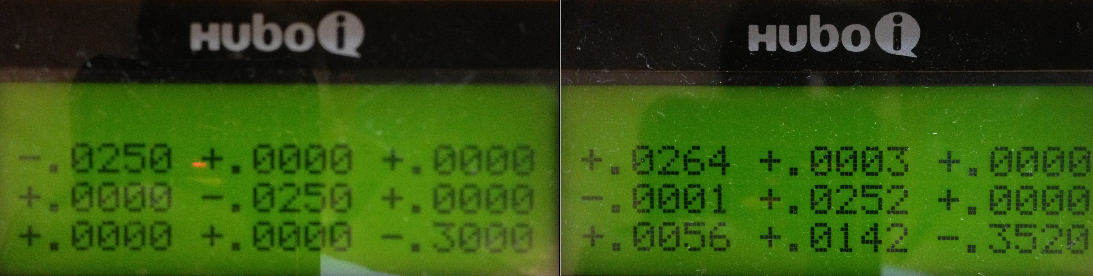
\includegraphics[width=15cm]{resources/ft-scaling-matrices}
\end{itemize}

\section*{September 23}
\subsection*{Biped Walking Status}
\begin{table}[h]
    \centering
    \caption{Biped ZMP Walking Tuning of ZMP X Offset}
    \begin{tabular}{|c|c|c|c|c|c|p{5cm}|} \hline
    \multicolumn{7}{|c|}{ZMP Walking Parameters} \\ \hline
        com\_z & fixed\_com\_offset\_z & zmp\_off\_x & zmp\_off\_y & Steps & step\_length & Results \\ \hline
        0.84 & 0.295 & 0.02 & 0.010 & 16 & 0.1 & Good \\ \hline
        0.84 & 0.295 & 0.026 & 0.009 & 16 & -0.1 &  \\ \hline
        0.84 & 0.295 & 0.02 & 0.009 & 16 & side 0.3 &  \\ \hline
    \end{tabular}
\end{table}

\section*{September 19}
\subsection*{Biped Walking}
Tuning COM Height, zmp\_offset\_x and zmp\_offset\_y with battery
\begin{table}
    \centering
    \caption{Biped ZMP Walking Tuning of COM Height \& ZMP Y Offset}
    \begin{tabular}{|c|c|c|c|c|c|p{5cm}|} \hline
    \multicolumn{7}{|c|}{ZMP Walking Parameters} \\ \hline
        com\_z & fixed\_com\_offset\_z & zmp\_off\_x & zmp\_off\_y & Steps & step\_length & Results \\ \hline
        0.82 & 0.275 & 0.02 & 0.007 & 16 & 0.1 & out of phase. Not enough sway, or COM too heigh \\ \hline
        0.82 & 0.275 & 0.02 & 0.008 & 16 & 0.1 & \textbf{Good} \\ \hline
        0.82 & 0.275 & 0.02 & 0.008 & 25 & 0.1 & \textbf{Good} \\ \hline
        0.82 & 0.275 & 0.02 & 0.009 & 16 & 0.1 & \textbf{Good} \\ \hline
        0.82 & 0.275 & 0.02 & 0.010 & 16 & 0.1 & No Good at end \\ \hline \hline
        0.84 & 0.295 & 0.02 & 0.002 & 16 & 0.1 & Too little sway \\ \hline
        0.84 & 0.295 & 0.02 & 0.004 & 16 & 0.1 & Too little sway \\ \hline
        0.84 & 0.295 & 0.02 & 0.006 & 16 & 0.1 & Good but too little sway at beginning \\ \hline
        0.84 & 0.295 & 0.02 & 0.007 & 16 & 0.1 & Good but ankles too a bit out of synch \\ \hline
        0.84 & 0.295 & 0.02 & 0.008 & 16 & 0.1 & \textbf{Good} \\ \hline
        0.84 & 0.295 & 0.02 & 0.009 & 16 & 0.1 & \textbf{Good} \\ \hline
        0.84 & 0.295 & 0.02 & 0.010 & 16 & 0.1 & \textbf{Good}. End a bit shaky \\ \hline
        0.84 & 0.295 & 0.02 & 0.010 & 25 & 0.1 & \textbf{Good} \\ \hline
        0.84 & 0.295 & 0.02 & 0.011 & 16 & 0.1 & \textbf{Good} \\ \hline
        0.84 & 0.295 & 0.02 & 0.012 & 16 & 0.1 & \textbf{Good} \\ \hline
        0.84 & 0.295 & 0.02 & 0.013 & 16 & 0.1 & No Good \\ \hline \hline
        0.85 & 0.305 & 0.02 & 0.010 & 16 & 0.1 & Good \\ \hline
        0.85 & 0.305 & 0.02 & 0.011 & 16 & 0.1 & Too much sway \\ \hline \hline
        0.86 & 0.315 & 0.02 & 0.008 & 16 & 0.1 & No Good. Too little sway \\ \hline
        0.86 & 0.315 & 0.02 & 0.010 & 16 & 0.1 & \textbf{Good} \\ \hline
        0.86 & 0.315 & 0.02 & 0.011 & 16 & 0.1 & Okay \\ \hline
        0.86 & 0.315 & 0.02 & 0.012 & 16 & 0.1 & \textbf{Good} \\ \hline
        0.86 & 0.315 & 0.02 & 0.013 & 16 & 0.1 & Good till end \\ \hline
        0.86 & 0.315 & 0.02 & 0.014 & 16 & 0.1 & No Good \\ \hline \hline
        0.90 & 0.355 & 0.02 & 0.012 & 16 & 0.1 & Pretty Good \\ \hline
        0.90 & 0.355 & 0.02 & 0.013 & 16 & 0.1 & \textbf{Good} \\ \hline
        0.90 & 0.355 & 0.02 & 0.014 & 16 & 0.1 & \textbf{Good} \\ \hline
        0.90 & 0.355 & 0.02 & 0.015 & 16 & 0.1 & \textbf{Good} \\ \hline
        0.90 & 0.355 & 0.02 & 0.016 & 16 & 0.1 & \textbf{Good} \\ \hline
        0.90 & 0.355 & 0.02 & 0.017 & 16 & 0.1 & No Good \\ \hline \hline
        0.94 & 0.395 & 0.02 & 0.015 & 16 & 0.1 & No Good \\ \hline
        0.94 & 0.395 & 0.02 & 0.013 & 16 & 0.1 & Almost Okay \\ \hline
        0.94 & 0.395 & 0.02 & 0.014 & 16 & 0.1 & Pretty Good \\ \hline
        0.98 & 0.435 & 0.02 & 0.013 & 16 & 0.1 & Too little sway \\ \hline
        0.98 & 0.435 & 0.02 & 0.014 & 16 & 0.1 & Too little sway \\ \hline
        0.98 & 0.435 & 0.02 & 0.015 & 16 & 0.1 & Too little sway \\ \hline
        0.98 & 0.435 & 0.02 & 0.016 & 16 & 0.1 & Pretty Good \\ \hline
        0.98 & 0.435 & 0.02 & 0.017 & 16 & 0.1 & Pretty Good. Sketchy start \\ \hline
        0.98 & 0.435 & 0.02 & 0.018 & 16 & 0.1 & \textbf{Good} \\ \hline
        0.98 & 0.435 & 0.02 & 0.019 & 16 & 0.1 & Pretty Good \\ \hline
        0.98 & 0.435 & 0.02 & 0.020 & 16 & 0.1 & No Good. But better start \\ \hline
    \end{tabular}
\end{table}

\begin{table}
    \centering
    \caption{Biped ZMP Walking Tuning of ZMP X Offset}
    \begin{tabular}{|c|c|c|c|c|c|p{5cm}|} \hline
    \multicolumn{7}{|c|}{ZMP Walking Parameters} \\ \hline
        com\_z & fixed\_com\_offset\_z & zmp\_off\_x & zmp\_off\_y & Steps & step\_length & Results \\ \hline
        0.84 & 0.295 & 0.02 & 0.009 & 16 & 0.1 & Good \\ \hline
        0.84 & 0.295 & 0.026 & 0.009 & 16 & -0.1 & Good \\ \hline
        0.84 & 0.295 & 0.02 & 0.009 & 16 & side 0.3 & Good \\ \hline
    \end{tabular}
\end{table}

\section*{September 18}
\subsection*{Landing Controller}
\begin{table} 
    \centering
    \caption{Landing Controller Gains and Results}
    \begin{tabular}{|c|c|c|c|c|c|} \hline
    \multicolumn{6}{|c|}{Landing Controller} \\ \hline
        Tp & $\zeta$ & M & K & Q & Result \\ \hline
        0.6 & 0.999 & 1.0 & 13715 & 234 & Terrifying shudders \\ \hline
        N/A & N/A & 5.0 & 20000 & 3000 & Slow oscillations \\ \hline
        2.2 & 0.999 & 25 & 25000 & 16000 & Better but oscillated too soon \\ \hline
        N/A & N/A & 55.0 & 25000 & 4000 & Good \\ \hline
    \end{tabular}
\end{table}


\section*{August 30}
\subsection*{Todo}
\begin{itemize}
  \item Changed convergence norm in Walker.cpp (\textbf{DONE}) and test
  \item Add checkbox to walk panel for specifying whether or not to keep the current arm positions during walking.
  \item Add ability to go to biped from current joint angles??
  \item Fix waist control in rviz panel.
  \item Why is CAN dying when we kill the motor power?
  \item Fix interpolation / Add joint control as an option
  \item Add goto last sent command angles
  \item Add goto home angles command
  \item Visualize state and plan simultaneously
\end{itemize}
\subsection*{Status}
\begin{itemize}
  \item Fixed static balancing for when the head is on.
  \newline
  \begin{figure}[h]
  \centering
  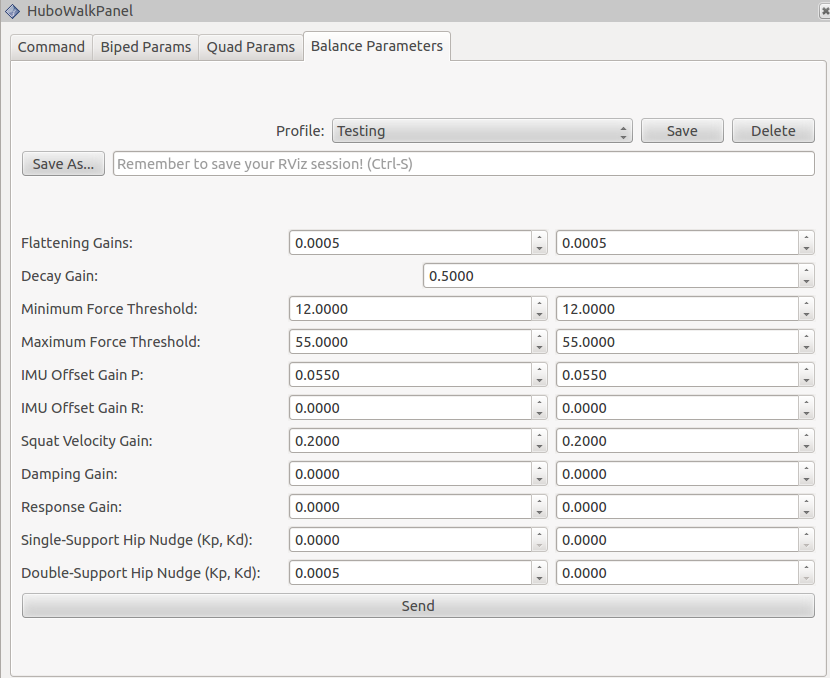
\includegraphics[width=10.0cm]{resources/static-balance-gains-with-head}
  \end{figure}
\end{itemize}

\section*{August 29}
\subsection*{Status}
\begin{itemize}
  \item Got the teleop pipeline running on my computer.
  \item Updated mission manual with rviz configuration instructions for the teleop stuff
  \item Almost done making it so we can walk with the last arm positions (ie. we can walk while holding things).
\end{itemize}

\section*{August 26}
\subsection*{Status}
\begin{itemize}
\item Tested biped/quadruped transitioning and quadruped walking on the robot. Everything worked as expected.
\item Updated master branches to include biped/quadruped stuff on hubomz and hubo\_walk.
\end{itemize}

\section*{August 24}
\subsection*{Joystick Walking Outline}
\textbf{zmp-daemon}
\begin{itemize}
    \item receive walk command
    \item generate n-sec zmp trajectory
    \item mark double-support time in generated trajectory, T1. 
    \item repeat
\end{itemize}
\textbf{Walker}
\begin{itemize}
    \item receive zmp trajectory which consists mainly of an array or ZMPReferenceContexts. 
    \item run zmp-preview
    \item run COM IK
    \item execute joint trajectory
\end{itemize}

\section*{August 22}
\subsection*{Status}
\begin{itemize}
\item Biped and Quadruped walking and transitioning works completely with forward/backward/sidestepping/turning-in-place. Just need to run a full test on the robot.
\item
\end{itemize} 
\subsection*{Todo (Next Week)}
\begin{itemize}
\item Clean up Walker and adjust it to use the control-daemon's trajectory mode.
\item Look into Yungbum's biped walking.
\item Add landing controller, which just requires adding single-support phase logic to my impedance controller, which is already written but untested on the robot.
\end{itemize}

\section*{August 21}
\subsection*{Status}
\begin{itemize}
\item Fixed Quadfootstep functions to account for current orientation of end-effectors.
\item Biped and Quadruped walking and transitioning works with forward/backward/sidestepping/turning-in-place. But quaddemo sidestepping doesn't work any more. Need to fix.
\end{itemize}

\section*{August 19}
\subsection*{Status}
\begin{itemize}
\item Tested transition between biped and quadruped (both directions) and walking in quadruped, all in the same run. It worked fine, but just need to slow down transition times in the parameters. Already done.
\newline
\begin{figure}[h]
\centering
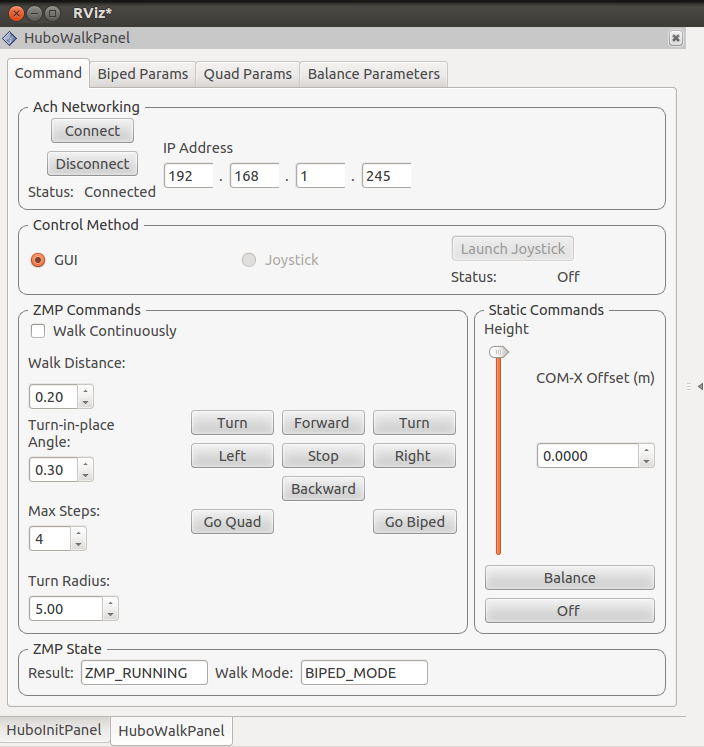
\includegraphics[width=8.0cm]{resources/HuboWalkPanel01}
\end{figure}
\newline
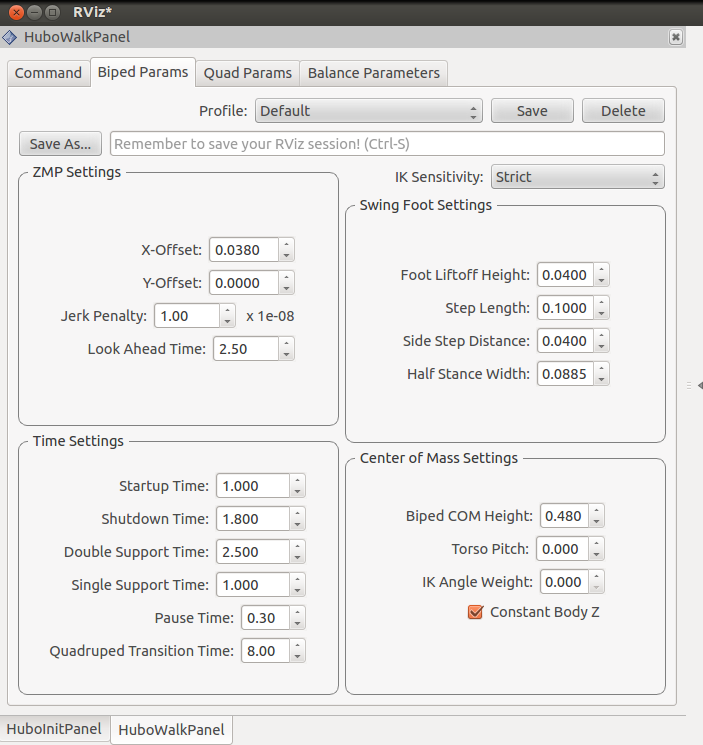
\includegraphics[width=8.0cm]{resources/BipedParams01}
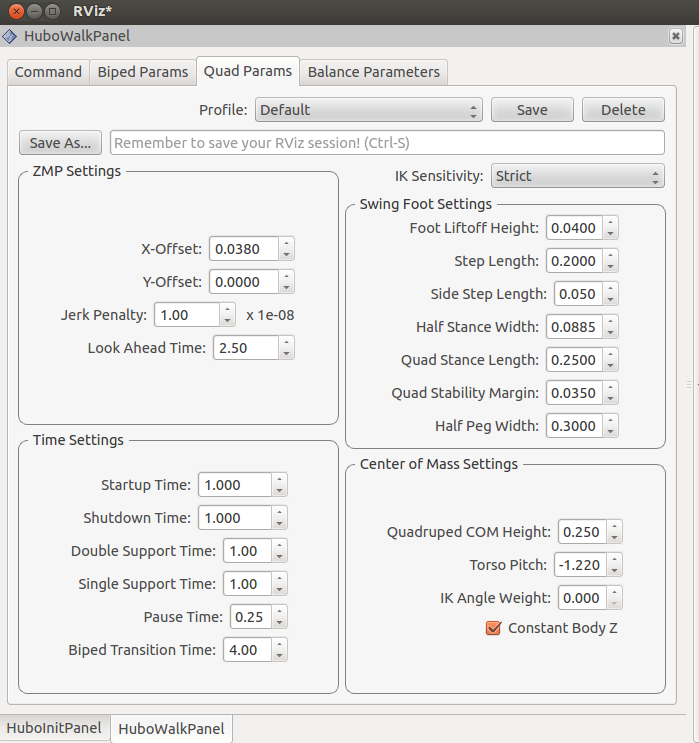
\includegraphics[width=8.0cm]{resources/QuadParams01}
\end{itemize}

\section*{August 16}
\subsection*{Issues Encountered}
\begin{itemize}
\item Walk Mode wasn't MODELESS on startup. This was because the hubo-zmp-state channel wasn't being destroyed every time.
\item When transitioning to biped or quadruped the zmp/com moves right just slightly when centering zmp in bipedSupport. I may have fixed this by changed how I calculate the state.body\_pos in makeBipedStartRef() function in zmpwalkgenerator.cpp.
\end{itemize}

\section*{August 15}
\subsection*{Status}
\begin{itemize}
\item Loaded wrist boards with new firmware from KAIST. It was Version MOT-120701, now it's Version MOT-307250.
\item Reconnected Left wrist/fingers board CAN cable.
\item Tightened finger cable in right middle finger so it properly homes and opens now.
\end{itemize}

\section*{August 06}
\subsection*{Status}
\begin{itemize}
\item If I put quadwalking into the GOTO\_QUADRUPED if statement and add in a centerZMP to biped support with emitTrajectory in between the foot step generation and the lerping, it works perfectly. But when I put the centeringZMP and lerping and foot steps into the quad walking if statement it says there's a jump in LSY.
\end{itemize}

\section*{July 30}
\subsection*{Status}
\begin{itemize}
\item Almost done adding Quadruped ZMP parameters tab to hubo\_walk. Grey and I also fixed hubo\_walk so that if the user doesn't have hubomz, then it won't load the ZMP Parameters tab.
\item Added in zmp\_state channel to the zmp-daemon to tell the hubo\_walk panel what the zmp-daemon is doing.
\item Fixed the transitions between quadruped and biped based on Matt's latest bug fixes and discussion with him.
\end{itemize}
\subsection*{Tomorrow}
\begin{itemize}
\item Finish adding quadruped tab and zmp-daemon state to hubo\_walk panel.
\item Finish writing zmp-daemon logic and test with zmpgui.
\end{itemize}
\subsection*{ZMP-DAEMON LOGIC}
\begin{itemize}
\item Start in zero position.
\item If GOTO\_QUADRUPED, Lerp(linearly interpolate) to quad support pose.
\item For QUADRUPED to BIPED, Lerp to zero position, then Lerp to biped support pose.
\item If GOTO\_BIPED, Lerp to biped support pose.
\item For BIPED to QUADRUPED, Lerp to zero position, then Lerp to quad support pose.
\end{itemize}

\section*{July 29}
\subsection*{Status}
\begin{itemize}
\item Merged the golems and swatbotics hubomz repositories to match, which will help us use each other's code and make things easier in the future. The plan is to only send pull requests to Matt from a branch on the golems repo or from a new branch on the swatbotics repo, but he doesn't want us push directly to his master.
\item Helped Matt find some bugs in his code that were making the merge of the quadwalk stuff into zmp-daemon difficult.
\item Retested the static balancing and discussed with Jim about the best approach for using static balancing for his WPI's valve-turning task. We definitely need to add some dampening and tune gains better. We are still trying to get info from Yungbum about his dampening controller, but it's difficult to get anything out of him for some reason. Are current idea is for WPI to generate an upper body trajectory, plus a torso angle trajectory that we can follow, and maintain as an error term in the balance daemon.
\end{itemize}

\section*{July 25}
\subsection*{Status}
\begin{itemize}
\item Got transition from biped to quadruped stance working in zmp-daemon. Transition back to biped seems to get generated in zmp-daemon, but zmpgui isn't showing any movement, so I am currently debugging this.
\item Helped Grey test the gravity compensation. Torque calculations and amp to pwm duty conversion/interpolation seems to check out just fine. Grey talked to Yungbum late in the day and got some insight that should help.
\item Matt derived the analytical IK for the arm with the elbow offset included. Just need to add handling of singularities.
\item Demoed Hongfei's keyboard teleop program for quadruped walking to a visitor.
\item Helped Rob and Yungbum weigh Hubo with a fish scale. Total mass without the battery is 49.8 kg.
\end{itemize}

\section*{July 24}
\subsection*{Status}
\begin{itemize}
\item Added buttons to hubo\_walk panel for transitioning to and from quadruped stance.
\item Refactored zmp-daemon code for ease of understanding and adjusting.
\end{itemize}

\section*{July 23}
\subsection*{Status}
\begin{itemize}
\item Finished merging Matt's quadruped code into the zmp-daemon repo, so zmp-daemon, zmpdemo and quaddemo all work. Next step is to add a quadruped option in zmp-daemon and integrate into the hubo\_walk rviz panel.
\item Helped Hongfei and Tae-gu run and debug quadruped teleop with the keyboard and hubo-read-trajectory, with Grey's awesome help.
\end{itemize}

\section*{July 22}
\subsection*{Status}
\begin{itemize}
\item Started verifying impedance controller but discovered zmp-daemon uses a model that has a very inaccurate mass, which caused the expected forces to be way too small. So I will finish merging Matt's newest hubomz into zmp-daemon and then get back to verifying the impedance controller.
\end{itemize}

\section*{July 21}
\subsection*{Status}
\begin{itemize}
\item Finished writing the workspace impedance controller for balancing. Need to test carefully.
\item Taught Hongfei git, and proof read his quadwalk teleop program, and helped him test it on the robot.
\item Compared analytical and iterative FK/IK for the arms and found them to be almost the same.
\item Worked with team to run teleop demo of picking up the drill.
\end{itemize}

\section*{July 20}
\subsection*{Status}
\begin{itemize}
\item Hip nudging during static balancing works now. We need to tune the gains and think of ways to make it better.
\newline Hip nudging gains:
\begin{itemize}
\item Flattening: 0.003
\item IMU Gain: 0.012
\item DS Hip Ndg: 0.0005
\item Squat Vel: 0.2
\end{itemize}
\item Added to the hubo\_walk rviz panel a setting for center of mass offset in the x-direction for static balancing. The desired torque for the hip nudging is computed by multiplying the desired center of mass offset by the mass of the robot, taken from DrcHuboKin.
\item Added installation and uninstallation to the CMakeLists.txt in hubo-motion-rt.
\item Merged my hipVelocityIK branch into master on hubo-motion-rt.
\item Tomorrow's plan is to check the error in the analytical IK for the arms due to the elbow offset and compare with the iterative IK, and investigate correcting the analytical IK. Also I will test my impedance controller for the legs.
\end{itemize}

\section*{July 19}
\subsection*{Status}
\begin{itemize}
\item Fixed the leg lengths in huboLegIK to be the same as in the FK, so now it works fine.
\item Tested the FK and IK in Hubo\_Control on the new Hubo, and it works now.
\item Tested the hip velocity IK on the new Hubo and it worked. We just need to replace the current version with Grey's new derivation which doesn't make assumptions about the leg lengths.
\item Successfully static balanced after switching the signs on the torque readings in the balance daemon, because the default on the boards is reversed.
\newline Should we switch this in hubo-ach?
\item I will test the hip nudging integrated into the static balancing tomorrow morning.
\end{itemize}
\subsection*{Misc}
\begin{itemize}
\item Helped Hong Fei set up the golems version of hubomz in order to learn how the hubo\_walk panel in rviz works and to look at the footprint generation for turning in place and sidestepping.
\item Helped Yung get further on the end-effector parsing.
\end{itemize}

\section*{July 18}
\subsection*{Status}
\begin{itemize}
\item Wrote a controller for static balancing that moves to hips along the x-y plane with a velocity proportional to the error in the ankle torque sensors. This complements the other two controllers for static balancing in order to counter external forces acting on the robot due to such things as picking up rubble or a drill. Will test tomorrow morning.
\item Wrote test program to verify the leg position FK/IK and hip velocity IK on the new robot. I will also compare with RobotKin's damped least square IK. Will test tomorrow morning before testing static balancing with the new hip nudging controller.
\item Fixed Hubo\_Control's leg FK and IK to give identity when the leg joints are all at zero.
\item Helped Yung understand how to parse his end-effector trajectories file in C++ and execute it on the robot.
\end{itemize}

\section*{July 17}
\subsection*{Status}
\begin{itemize}
\item Merged the quadruped branch into our golems master branch of hubomz. Quaddemo works and zmp-daemon starts but I need to fix my rviz stuff in order to test zmp-daemon fully.
\item Tae-goo and I ran the quadruped walking on Hubo on the rough terrain mockup for 12 steps, just on the flat section. It worked just fine. Next step is to add manual footstep placement to try and walk up the wooden platforms in the mockup.
The video is located at \href{http://www.youtube.com/watch?v=zqZra1Jmt9g&feature=youtu.be}{Quadruped Walking}
\item Met with the controls discussion group. Jim from WPI is working on the operational space control, Kiwon from Drexel is working on a way to have Hubo slide over to the driver seat in the vehicle without drawing too much current, Ben from Columbia thinking about the best way to manipulate the hose for attatchment.
\begin{itemize}
\item Kaist's Compliance Control (Some boxes missing for feedback using the encoders)
\newline 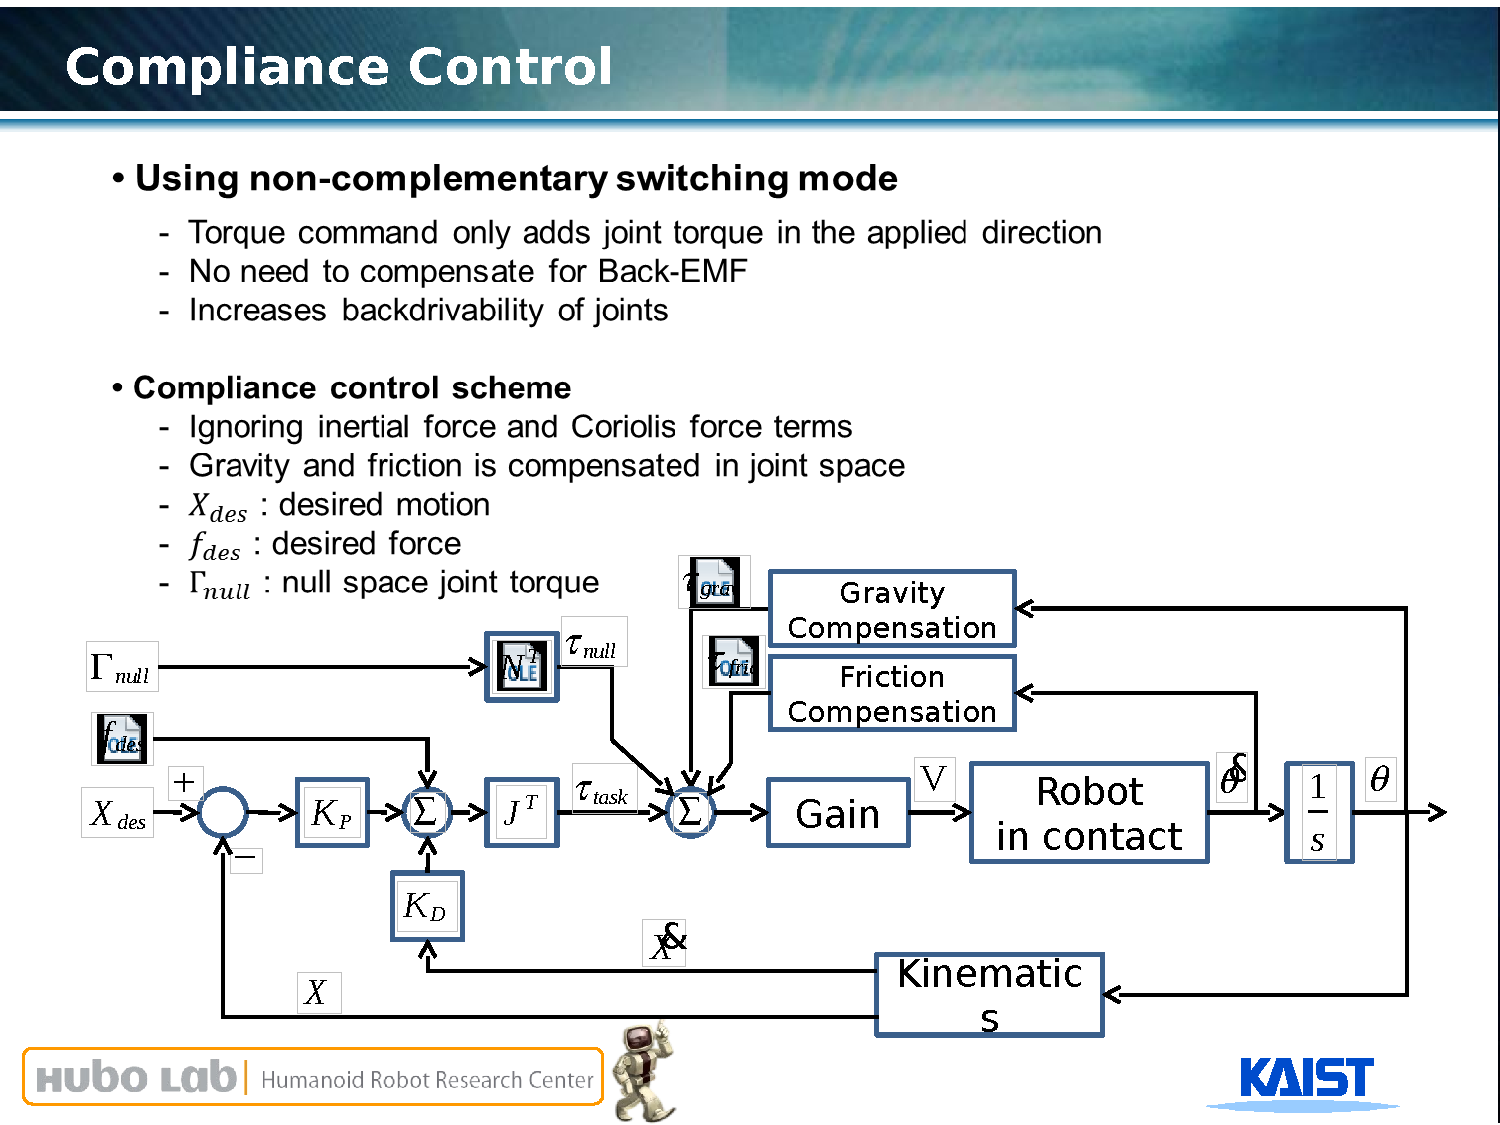
\includegraphics[width=14.0cm]{resources/compliance-control}
\end{itemize}
\end{itemize}

\section*{July 16}
\subsection*{Status}
\begin{itemize}
\item I helped Matt run his new quadruped zmp walking demo by having it write the trajectory to a text file and then running it using hubo-read-trajectory. It worked flawlessly after changing the peg lengths in the model. We performed 4 steps and 12 steps at 25, 50, 100 and 200 Hertz.
\item I started merging his quadruped walking code into our hubomz. Plan for tomorrow is to have zmp-daemon working for either biped or quadruped walking.
\item I explained hubomz and the whole zmp walking pipeline to Hong Fei from OSU and Tegu from Drexel, who will adopt hubomz for quadruped walking. We outlined a longterm plan to get to generating trajectories online potentially using feedback from the force/torque sensors to compute the actual zmp error, and specifying individual footsteps on the fly, which would eventually, hopefully beed done using vision and a footstep planner.
\item Explained to Yung, Kiwon's apprentice, how to go about converting Kiwon's Matlab vehicle ingress planner and the Rainbow code that takes the end-effector trajectories and computes joint angles, into C++ or Python using hubo-ach.
\item Helped Indiana and Purdue run their stair-climbing trajectory, since Hubo has been breaking a lot from their experiments. The right hip pitch was loose when they initial were going to try to climb the stairs, but I found some loose screws inside the hip, which after tightened seemed to fix the problem. Kiwon apparently has known about this problem and will need to disassemble the hip sometime to tighten everything down.
\end{itemize}

\section*{July 15}
\subsection*{Status}
\begin{itemize}
\item Wrote a workspace impedance controller for the legs, which accounts for $\tau_x$, $\tau_y$ and $F_z$. Will verify and debug (if necessary) tomorrow before testing.
\item Matt showed me what he changed in zmpdemo to create the quadruped version, quaddemo. I also learned how to run it and generate text file trajectories in order to test on Hubo using Dan's hubo-read-trajectory. I plan to test it tomorrow since Matt will not be in the lab.
\item Helped Rob load his new home parameters on drc-hubo-beta-2.
\end{itemize}

\section*{July 14}
\subsection*{Status}
\begin{itemize}
\item Tried to create a swing foot trajectory function that is parameterized by desired acceleration in the z-direction. Having trouble determining a good method of getting desired acceleration while maintaining desired single-support time.
\item Took apart the wrist with Ben and Grey to figure out why the left wrist stopped working. After Ben gave the LSR a negative reference and banged it into the left knee, it only would rotate 30 degrees. We ran out of time and just put it back together. Kiwon fixed it on 7/15.
\end{itemize}

\section*{July 12}
\subsection*{Status}
\begin{itemize}
\item Added derivative term to the hip nudging controller and tested it. Grey and I tried tuning the gains some and nothing dampened the oscillations, and at one point we brought the D-term higher than the P-term which resulted in rapid instability.
\item Finished 7/10 tasks \#1, 2, and 4.
\item Learned how to use Matt's hubo-logging repo, which includes a logger and a plotter, which is really useful.
\end{itemize}
\subsection*{Tasks}
\begin{enumerate}
\item Make a swing foot trajectory function that has deceleration parameterized.
\item Write controller that adjusts the hip height based on swing foot landing force to account for early landing or overshooting the stance foot.
\item Weigh the robot with and without the battery.
\end{enumerate}

\section*{July 11}
\subsection*{Status}
\begin{itemize}
\item Matt, Grey and I found some bugs in the Walker.
\begin{enumerate}
\item We were modifying the trajectory elements that we eventual recycle. We changed this so that we are making a copy before modifying and setting the joint angles.
\item We had the setJointVelocity() function after the passJointAngle(), so passJointAngle() was sending the joint angle passed the control daemon and into hubo-daemon, but setJointVelocity() was changing the control mode to velocity mode, and thus we were just running in velocity mode with a constant error, causing the feet to shoot back endlessly.
\item The NANs turned out to be from hubo\_walk because the balCmd struct was not being memset, and the balance-daemon supposedly static balances while waiting for a walk trajectory, and when it received the cmd.height from the balCmd channel, it was NAN and used to calculate the leg joint velocities, and therefore sending the control-daemon NANs. This fixed.
\end{enumerate}
\item Tested nudging of the hips while standing still and it worked well, but changing the gain a bit caused some oscillation due to only using a proportional gain at the moment.
\item Tested nudging while walking in place, but it seemed to be worse than the other day. Definitely need to implement landing control now.
\newline 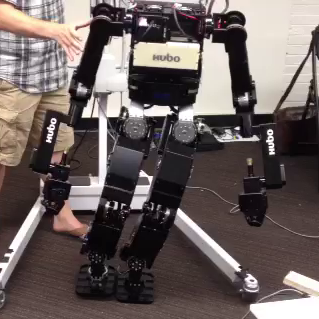
\includegraphics[width=5.0cm]{resources/walking-in-place-fail}
\item Tested balancing on one leg using nudging control, but it also had oscillation. We need damping in the legs using possibly impedance control.
\end{itemize}

\section*{July 10}
\subsection*{Status}
\begin{itemize}
\item I spent much of the day helping people learn how to use the robot, helping them run their trajectories and supervised them, as well as debugging some people's code. Fortunately, one of these was Ben from WPI, who is now already using the hubo\_init panel. It's good that they are testing because I don't think they've ever run anything on the robot and they are seeing how different it is from simulation.
\item Discovered a bug in Hubo\_Control with the convenience functions for getting the torque readings for the ankles while testing the nudgeHips function. The 'return' keyword was missing, which Grey caught.
\item I was unable to reproduce the NANs seen yesterday on either the half-Hubo or beta-1 Hubo. I started testing the nudgeHips() controller but then ran into the sensor readings problem above.
\item I tested the joint-manip-test on the half-Hubo because Andrew was having issues with the right arm responding and we discovered that the interrupt flag need to be set to true. I also wrote a version of the program that brings the arms back to zero position for convenience.
\item I saved a version of the drc-hubo-joint table for the half-Hubo that only has the existing and working joints set to active. For the time being this can just be vim diffed with the one installed to /etc/hubo-ach/drc-hubo-beta.joint.table.
\item Discovered that the F/T sensors in the wrists were not reporting any values in hubo\_init or my sensors program. I will verify this on beta-1 and beta-2 (which has the F/T sensors working in the Rainbow code).
\end{itemize}
\subsection*{Tasks For Thursday \& Friday}
\begin{enumerate}
\item \textbf{(Done)} Finish testing/verifying the nudgeHips() walking controller, determine appropriate gains and test it during quasistatic walking with a slower single support phase.
\item \textbf{(Done)} Verify whether or not the F/T sensors are being read by hubo-ach correctly on beta-1 and beta-2 Hubo. \textbf{They are.}
\item Finish making CMAKE work with hubo-motion-rt.
\item Write an outline of what needs to change in hubomz to implement quadriped walking. \textbf{Matt will do it.}
\end{enumerate}

\section*{July 09}
\subsection*{Progress}
\begin{itemize}
\item Cleaned up nudgeHips() walking controller with Grey and Matt. Need to debug IK issues because the feet compensated way farther than they should have when we ran it in the air.
\item Tomorrow's plan is to finish debugging the NAN's in the control daemon, debug the IK, and test hip nudging with slowing walking speeds.
\end{itemize}
\subsection*{Status}
\begin{itemize}
\item Changed zmp-daemon and zmpgui to use pointers on the heap instead of primitives on the stack because the stack was being overflowed after increasing zmp traj ach channel size and zmp max traj size to accomodate slower walking gates.
\item Matt, Grey and I debugged some issues in the Walker's nudgeHips() controller, but got detoured due to CAN wire issues.
\begin{itemize}
\item When we homed once it worked. Homing the second time, the upper body didn't respond. The RWR motor control board CAN wire was getting pulled out or something during the first home, which caused the upper body to fail the second time around. This was repaired at the end of the day.
\item We tried after temporarily fixing the above issue and the legs stopped responding during the phase of getting into the initial position of the trajectory. Discovered that the control daemon was computing NANs somehow. Grey and I discovered some weird things going on using printfs but still haven't found the exact cause yet.
\end{itemize}
\end{itemize}

\section*{July 08}
\subsection*{Status}
\begin{itemize}
\item Figured out that the reason hubo\_walk was not working and during make, errors involving boost/operators.hpp and ros/console-brdige/console.h and LogLevel. The reason was because I moved 'include "Hubo\_Control.h"' from balance-daemon.cpp to balance-daemon.h, which include hubo.h which include syslog.h which has pound defines that conflict with ros. This is because hubo\_walk includes balance-daemon.h.
\end{itemize}

\section*{July 07}
\subsection*{Status}
\begin{itemize}
\item Calibrated Hubo's legs. Realized that Hubo doesn't hang level on the hoist, which can significantly affect calibration if using a level.
\item Tried balancing first and using the ankle roll offsets from the balancing in the Walker, but that didn't help things.
\end{itemize}

\section*{July 06}
\subsection*{Status}
\begin{itemize}
\item Determined that the jittery behavior when walking was due to using std::cerr instead of std::cout. This is because cerr is unbuffered and sends everything to the terminal immediately, causing a slowdown in the trajectory, where as std::cout buffers it and then sends a batch to the terminal. With std::cout it was much better, but possibly still affecting it a bit.
\item Tested quasistatic walking in place using the nudgeHips function (see June 03). Even after calibrating the feet some, it still had the same problem. Maybe more calibration is necessary. I believe that for such feedback control to work properly, the feet need to be flatten before walking, and then the offset used throughout the walking trajectory, otherwise there's no way to ensure the legs and ankles are perfectly calibrated and it won't happen again.
\end{itemize}
\subsection*{Ideas}
\begin{enumerate}
\item Always balance before walking and use ankle offsets in walking trajectory.
\begin{itemize}
\item Doing this as is would mean when walking started, Hubo would "jolt" a bit forward to get to the initial ZMP\_x offset, which is currently 0.04m. 
\item Or using the COM height and the ZMP\_x offset to compute the new desired IMU angle about the y (pitch) axis.
\end{itemize}
\item Use accelerometers in the feet to flatten the feet without affecting the body position.
\end{enumerate}

\section*{July 05}
\subsection*{Status}
\begin{itemize}
\item Added installation to the CMakeLists.txt in hubo-motion-rt, and also added an uninstall cmake file so you can now type 'sudo make uninstall' in the build directory.
\item Found old, uncorrected bug in control.table in hubo-motion-rt. The hip yaw and hip pitch for both legs were swapped, which affect how they get ordered in the leg joints arrays.
\item Updated Walker.cpp to adjust both legs in both single and double support, and tested it on Hubo without actually changing the trajectory, but somehow it caused some jittery behavior. I will investigate this tomorrow.
\item Added single and double support hip nudge gains to the hubo\_walk panel in rviz, and added the gains to the balance-daemon accordingly.
\item Updated leg lengths constants and limits in HuboKin.cpp and the control.table in hubo-motion-rt. 
\end{itemize}
\subsection*{Issues}
\begin{itemize}
\item Jittery behavior from nudgeHips() function in Walker.cpp.
\item zmpdemo.cpp has TopicUnaligned... eigen error in the gui demo section.
\item hubo\_init get ACH\_OVERFLOW from the hubo-state channel at times. Maybe a race condition since it uses threads.
\end{itemize}

\section*{July 04}
\subsection*{Status}
\begin{itemize}
\item Added nudgeHips() function to Walker.cpp.
\end{itemize}

\section*{July 03}
\subsection*{Status}
\begin{itemize}
\item Plan for walking:
\begin{enumerate}
\item Try quasistatic walking with 0 step height, with the battery in.
\item Try quasistatic walking with flattening of the feet.
\item Try dynamic walking with flattening of the feet.
\item Try running the zmp-daemon realtime using the force/torque sensor and maybe the accelerometer in the pelvis to determine the real ZMP and use that in the Preview Controller every timestep.
\end{enumerate}
\item 1. Quasistatic shifting back/forth worked very well without the battery.
\item 2. Quasistatic walking in place worked well, except that the miscalibration in the left ankle roll caused the robot to fall to the right during single-support, which then caused the dropping leg to hit the ground and push the robot over. But the right side was perfect. Another possible explanation that Grey mentioned was that the new adapter piece between the right F/T sensor and the ankle is a bit thicker (or the calibration of the legs are such that the body is leaning to the left) causing Hubo to lean to the left, which then causing him to fall right when he lifts his right leg.
\begin{itemize}
\item x-offset = 0.4m
\item y-offset = 0.0m
\item zmp-R = 1.00 x 10\^-8
\item lookahead time = 2.5s
\item startup = 1.0s
\item shutdown = 1.8s
\item double-support = 2.5s
\item single-support = 1.0s
\item pause time = 0.3s
\item step height = 0.06m
\item step distance = 0.0m
\item half stance width = 0.0885m
\item COM height = 0.45m
\item flattening gains = 0.001

\item decay gain = 0.5
\item min force threshold = 12.0N
\item max force threshold = 55.0N
\end{itemize} 
\item 3. Dynamic walking didn't work well with the various parameters Matt and I tried. Hubo's joint shifting and body leaning became out of phase by a step each time (ie. when his legs were such that they would make him shift left, he was leaning right on the right edge of his feet.).
\item Matt and I discussed the implementation of torque feedback to nudge the hips in the opposite direction of the falling and I will be ready to test it on Friday morning.

\begin{equation}
\begin{bmatrix}
f_x \\ 
f_y \\
f_z
\end{bmatrix}
=
\begin{bmatrix}
dt*K_p && 0 && 0 \\
0 && dt*K_p && 0 \\
0 && 0 && 0
\end{bmatrix}
\begin{bmatrix}
0 && 1 && 0 \\
-1 && 0 && 0 \\
0 && 0 && 0
\end{bmatrix}
\begin{bmatrix}
\tau_{x_{desired}} - \tau_{x_{measured}} \\
\tau_{y_{desired}} - \tau_{y_{measured}} \\
\tau_z = 0
\end{bmatrix}
\end{equation}

\begin{equation}
\begin{bmatrix}
iF_x \\
iF_y \\
iF_z
\end{bmatrix}
+=
\begin{bmatrix}
\cos(\theta_{HY}) && -\sin(\theta_{HY}) && 0 \\
\sin(\theta_{HY}) && \cos(\theta_{HY}) && 0 \\
0 && 0 && 1
\end{bmatrix}
\begin{bmatrix}
f_x \\
f_y \\
f_z = 0
\end{bmatrix}
\end{equation}

\begin{equation}
FootTF[LEFT] = legFK(qPrev[LEFT])
\end{equation}
\begin{equation}
FootTF[RIGHT] = legFK(qPrev[RIGHT])
\end{equation}

where $\tau_x$ and $\tau_y$ are the measured torques minus the expected torques for the x and y axes. $f_x$ and $f_y$ are the instantaneous (every 0.005s) x- and y- position offsets of the feet given the torque feedback error. $iF_x$ and $iF_y$ are the integrated x- and y- position offsets of the feet with the hip yaws taken into account. This then gets premultiplied by the TFs from the body to the feet to get the new feet positions, on which we run the IK to get the new leg joint angles that will nudge our hips to counter any falling motion.
If we integrate the body error, than we can save the accumulated error in the legs joint with two numbers and apply IK to.
\end{itemize}
\subsection*{Issues}
\begin{itemize}
\item The left PC has login issues. To solve it, press Ctrl-Alt-F1 to go to the Terminal. Then type sudo chown groupname:username .Xauthority. Then press Ctl-Alt-F7 to go back to the login and try logging in.
\end{itemize}

\section*{July 02}
\subsection*{Status}
\begin{itemize}
\item Found a weird bug in zmpwalkgenerator.cpp, line 416 in github.com/swatbotics/hubomz/zmp/. If the center of mass IK fails then it gets the body transforms using the walker's local initContext, but it has not been set yet, so jvalues.size() = 0 and therefore the assert in KinBody::transforms() fails.
\item Tested quasistatic walking with 1.5 double-support time. When it first moved to the left foot it did well, but when it shifted to the right, it went way too fast and overshot and fell over. We presume this may be because the double-support time is too short, but just increasing this doesn't seem like a good idea.
\item Figured out that the footstep generation functions don't know anything about the zmp position so the final step ends with the body shifted to the side with the zmp\_y at it's max. So stayDogStay() using the shutdown\_ticks is necessary to bring the zmp\_y back to zero.
\item Tried much longer double-support time with quasistatic walking in place. The first shift to the left foot was perfect, but when Hubo put his right foot back down he fell off balance and then fell to the right as he shifted right. Will implement a feedback controller tomorrow.
\end{itemize}
\subsection*{Issues}
\begin{itemize}
\item In quasistatic mode the single and double support times need to be very long, which creates a very large trajectory, which currently overflows the ach channel. So we can either increase the ach channel size (temporary plan), or move onto atomic trajectories.
\end{itemize}

\section*{July 01}
\subsection*{Status}
\begin{itemize}
\item Worked with Matt and found bug in hubomz code in zmpwalkgenerator.cpp where the if else statements for pause\_time were switch, so it was interpolating the body rotation over the wrong number of iterations.
\item Tested quasistatic walking on DRC Hubo 1, but when he leaned over the left foot, he ended up falling to the left side. My deduction is that the model is not correct (ie. the center of mass is too low) which caused Hubo to lean to far and thus put his ACTUAL center of mass outside his support foot.
\item Parameters were: X-offset: 0.04, Startup time: 1.0, Shutdown time: 1.0, Double-support time: 0.9, Single-support time: 1.0, Pause time: 0.3, Step height: 0.1, Step distance: 0.22, Lateral distance: 0.0885, Center of mass height: 0.45.
\item I added a function to the Walker class in hubo-motion-rt called balanceAboveFoot that will hopefully help account for the inaccuracies in the model and allow for quasistatic working to work.
\end{itemize}
\subsection*{Issues}
\begin{itemize}
\item We discovered that the Force/Torque sensors in the ankles were reversed on all the signs when using Hubo-i, but when using hubo\_init, just the right ankle was incorrect.
\item Kiwon Sohn contacted KAIST and they said they purposely set the F/T sensors backwards and since defaulting to the stock firmware will revert them to being backwards, we should just change it in our code. This is not logical at all, but not much we can do about it now.
\end{itemize}

\section*{June 25}
\subsection*{Status}
\begin{itemize}
\item Ported our zmp-daemon code over to Matt's new hubomz repo which now works with the new DRC Hubo. Got everything working (ie. forward/backward, sidestepping and turning in place) except that there is something weird going on in the first step of the turn in place.
\item Currently the repo is forked to my user account "pvieira3".
\end{itemize}
\subsection*{Issues}
\begin{itemize}
\item Need to think about best and most logical way to use ZMPParams and where to put them. Currently I have put the ik\_sense and the walktype in zmp-daemon and zmpwalkgenerator includes zmp-daemon. This led to changing some lines in zmpdemo as well.
\item Need to fix turning in place.
\end{itemize}

\section*{June 22}
\subsection*{Status}
\begin{itemize}
\item Updated hubomz: merged grey/daemonize into master and cleaned up the code some.
\item Now using master for hubomz and hubo\_walk, manipulation for hubo-motion-rt and
develop for hubo-ach.
\item Push Hubo's plastic pieces back on and packed everything for Drexel.
\end{itemize}

\section*{June 21}
\subsection*{Status}
\begin{itemize}
\item On local PC start 'roscore' and 'rosrun rviz rviz'
\item On hubo-vision start 'roslaunch openni\_launch openni.launch'
\item 'export ROS\_MASTER\_URI=http://COMPUTER\_NAME:11311/'
\item On local PC run 'rosrun rqt\_reconfigure rqt\_reconfigure' and check the camera/driver depth\_registered box
\item On local PC run 'roslaunch hubo\_motion\_ros hubo\_manipulation.launch' (to see camera and hubo)
\item On local PC run 'rosrun hubo\_drc\_vision segment\_image'
\end{itemize}

\section*{June 20}
\subsection*{Status}
\begin{itemize}
\item Wrote a function to test the handle\_angles function in the manipulation-daemon and tested it. It worked fine.
\item Read through basic understanding of Point Cloud Library.
\item Wrote function to convert pcl PointCloud2 from camera to a PointXYZRGB and then compute the point cloud normals and store the two together as a PointXYZRGBNormal to be used for segmentation of planes
\end{itemize}

\section*{June 19}
\subsection*{Status}
\begin{itemize}
\item Added function in manipulation daemon to handle raw joint angles for the arms instead of poses, because the IK was coming up with different angles than what was put into the FK on the ROS side.
\item Change board limits for RSR and LSR so that going in toward Hubo's center the limit is 0.36 radians. Somehow they got messed up and were at 0.157 radians. Changed control.table to reflect this.
\item Went through ROS tutorials: "Services \& Parameters", "Using rqt\_console and roslaunch", "Using rosed to edit files in ROS", "Creating a ROS msg and srv", "Writing a Simple Publisher and Subscriber", "Examining the Simple Publisher and Subscriber", "Writing a Simple Service and Client", "Examining the Simple Service and Client".
\end{itemize}

\section*{June 18}
\subsection*{Status}
\begin{itemize}
\item Discovered control table has conservative limits on shoulder roll joints. Currently +/- 0.3, but really should be +/-0.4. Discuss reasons with Grey.
roslaunch hubo\_motion\_ros hubo\_state.launch.
\end{itemize}
\subsection*{Todo}
\begin{itemize}
\item Get more accurate TF to checkerboard (Add to code)
\item Change manip daemon to use joint angles
\item Write test code for joint angles manip cmd
\item Get better calibration points
\end{itemize}

\section*{June 16}
\subsection*{Status}
\begin{itemize}
\item Fixed bug in zmp-daemon which caused discontinuity
\item Got rid of unused code in zmp-daemon
\item Merged risky/daemonize into grey/daemonize
\end{itemize}

\section*{June 13}
\subsection*{Status}
\begin{itemize}
\item While testing current control using KAIST's method, Grey discovered that we'd been using Dan Lofaro's filter b/c in the control daemon use\_filter was set to false and then immediately set back to true.
\item This cause lots of distortion using a .25s window, which screwed up the timing of the zmp walking.
\item We tested trajectory without the filter and after fixing a bug it works fine now and the timing is accurate!
\end{itemize}

\section*{June 03}
\subsection*{Status}
\begin{itemize}
\item Started writing zmp atomic trajectories concept.
\item Basically, slice trajectories up into their individual steps so we can just piece them together. This way we can generate all atomic trajectories for each walk type all at once, and then use them on the fly, which gets rid of the generation time when changing directions.
\end{itemize}

\section*{June 01}
\subsection*{Status}
\begin{itemize}
\item Wrote preview controller for model that includes angular momentum. It's located in ZmpPreview.h in hubomz/src
\item Doesn't converge with current values
\end{itemize}

\section*{May 28}
\subsection*{Status}
\begin{itemize}
\item Changed zmp-daemon to send one trajectory and have zmpgui/walker reuse the periodic portion of it.
\item This decreased the cpu usage of zmp-daemon from 100\% to about 2\%.
\end{itemize}

\section*{May 13}
\subsection*{Status}
\begin{itemize}
\item Got OpenGL zmpgui to run trajectories continuously.
\end{itemize}

\section*{May 12}
\subsection*{Status}
\begin{itemize}
\item Added keyboard controls to zmp-daemon for walking forward/backward, sidestepping and turning.
\end{itemize}


\section*{May 11}
\subsection*{Issues}
\begin{itemize}
\item Walktype "canned" doesn't account for initial conditions. Need to get rid of it and use footstep.cpp walk functions
\item Where is best swap-in point? At end of double-support, have max CoM and joint velocities.
\end{itemize}
\subsection*{Thoughts}
\begin{itemize}
\item Use last ZMPReferenceContext element in the ref vector in walker after adding 2nd to last step as the initContext for the next trajectory.
\end{itemize}

\section*{May 10}
\subsection*{Issues}
\begin{enumerate}
\item Discovered ach doesn't work between computers with different architectures. Need to made struct variables uint\#, etc. and use \_\_attribute\_\_((packed))
\item Swapping in trajectories results in large joint velocities (ie. discontinuity). Something is wrong!
\end{enumerate}
\subsection*{Thoughts}
\begin{enumerate}
\item
\begin{itemize}
\item Change structs that we're passing over ach to \_\_attribute\_\_((packed)) and specify variable sizes using inttypes.h (ie. uint8)
\end{itemize}
\item
\begin{itemize}
\item Does walker modify joint angles at all?
\item Validate swap point inside zmp-daemon
\item Plot it
\end{itemize}
\end{enumerate}

\section*{May 09}
\subsection*{Status}
\begin{itemize}
\item Created walker flowchart and state machine
\newline 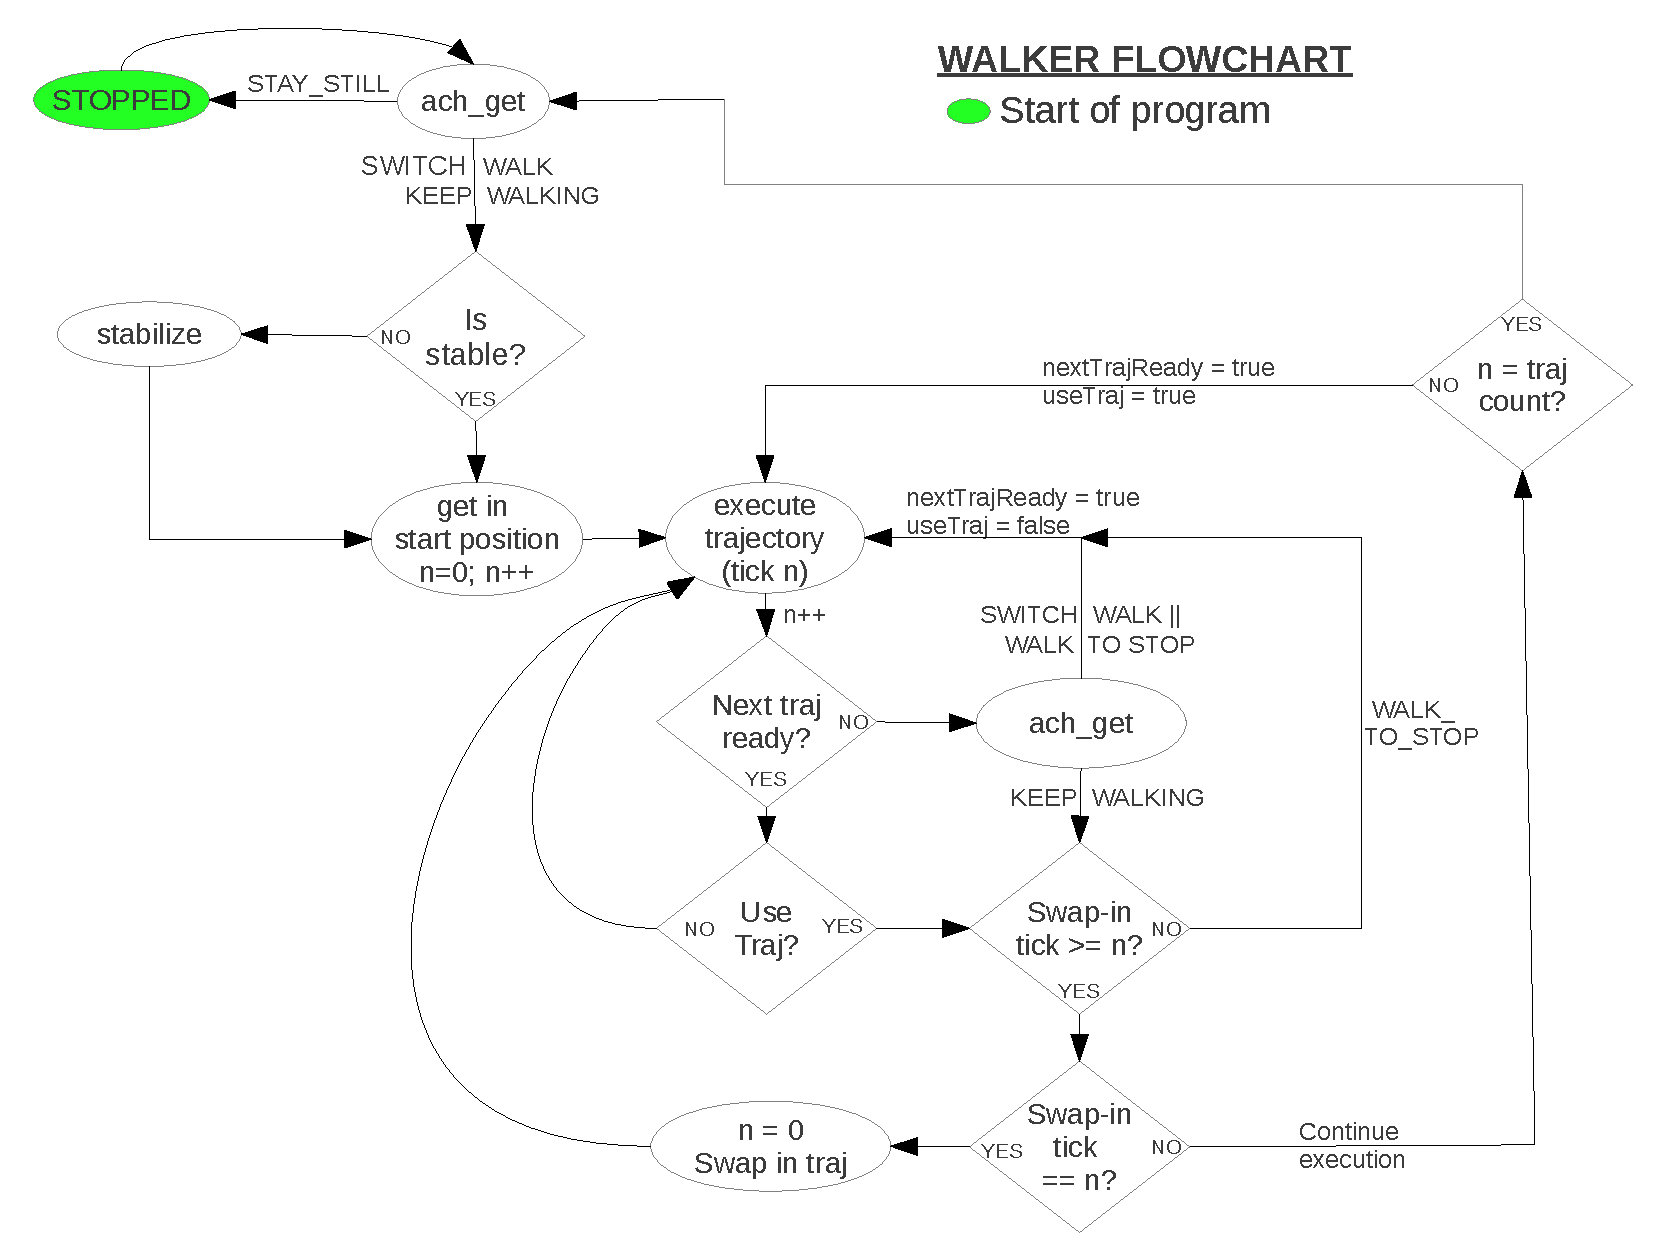
\includegraphics[width=\linewidth]{resources/walker-flowchart}
\end{itemize}

\section*{May  07}
\subsection*{Status}
\begin{itemize}
\item Made preliminary state machine for zmp-daemon and walker for continuous trajectory generation
\item Created zmpdemo flowchart
\newline 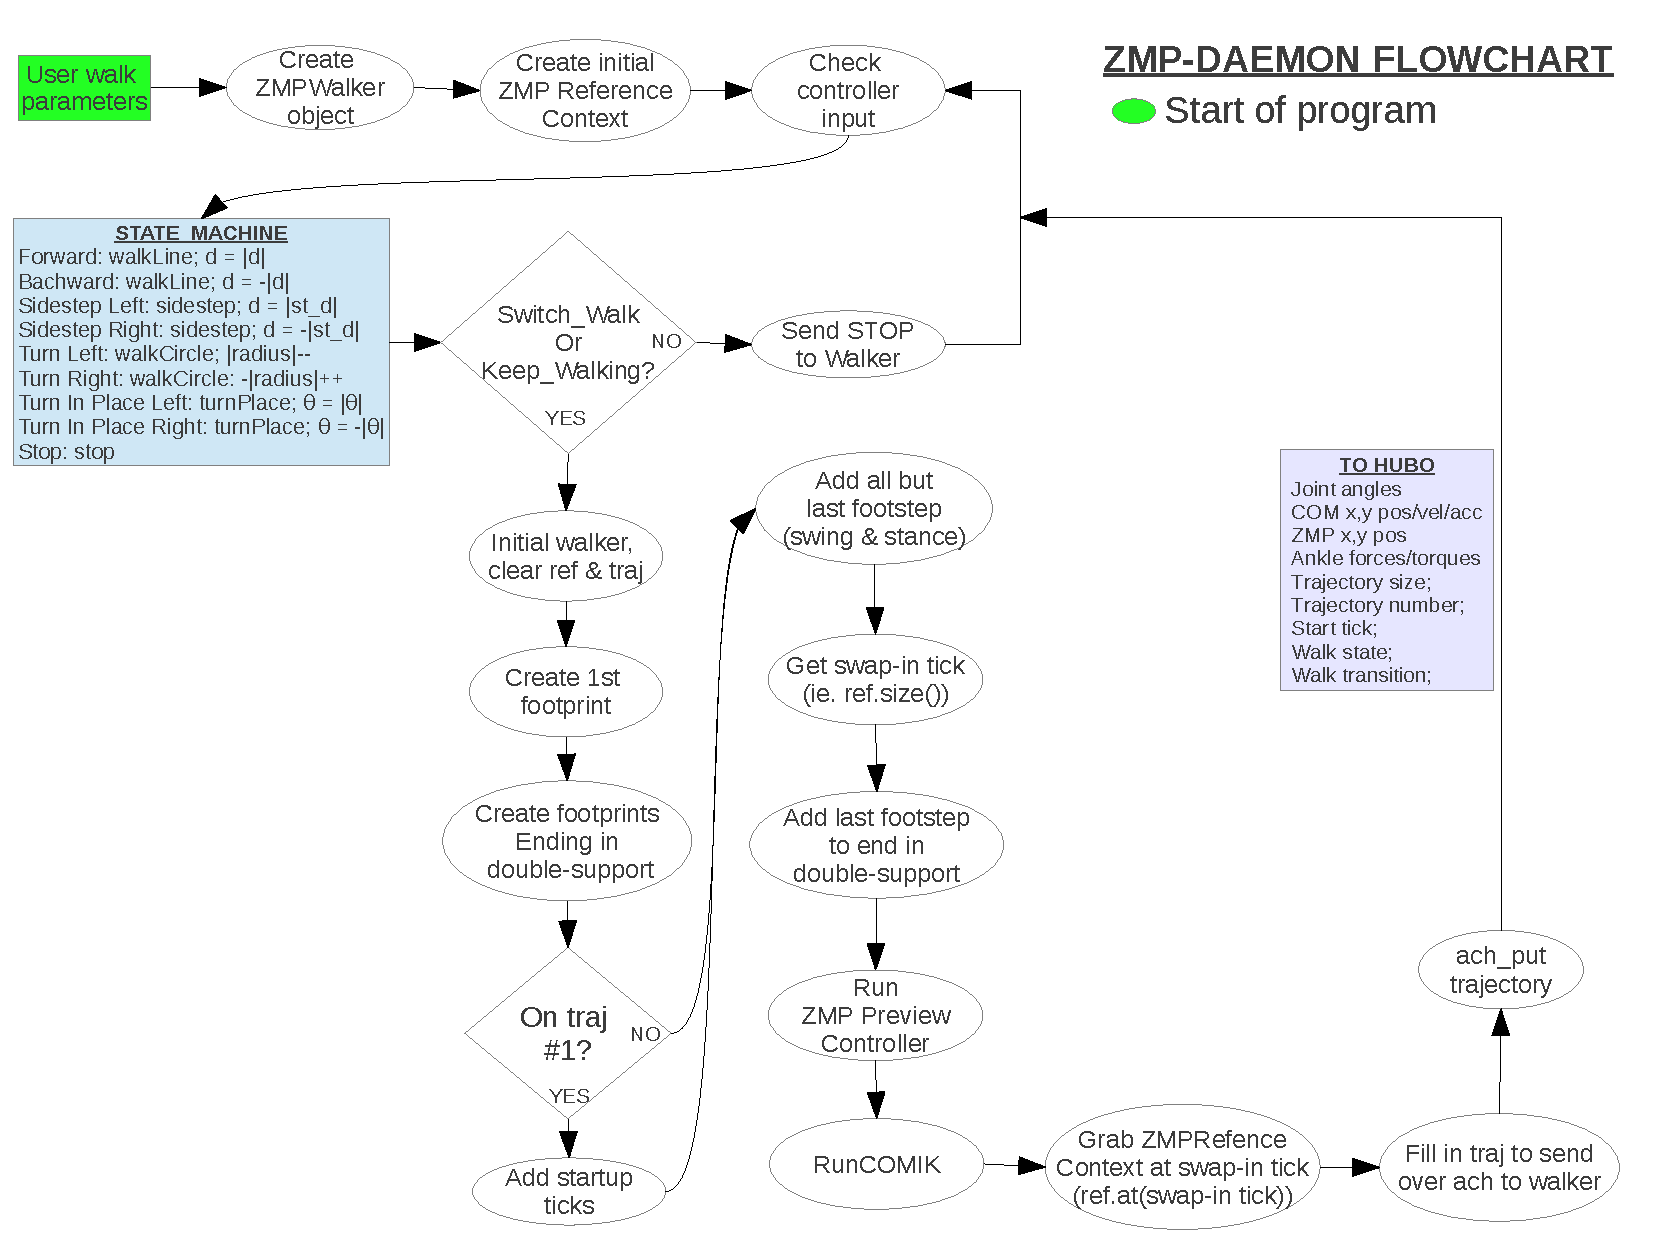
\includegraphics[width=\linewidth]{resources/zmp-daemon-flowchart}
\item Edited walking-pipeline and added diagram of continuous walking receding horizon
\newline 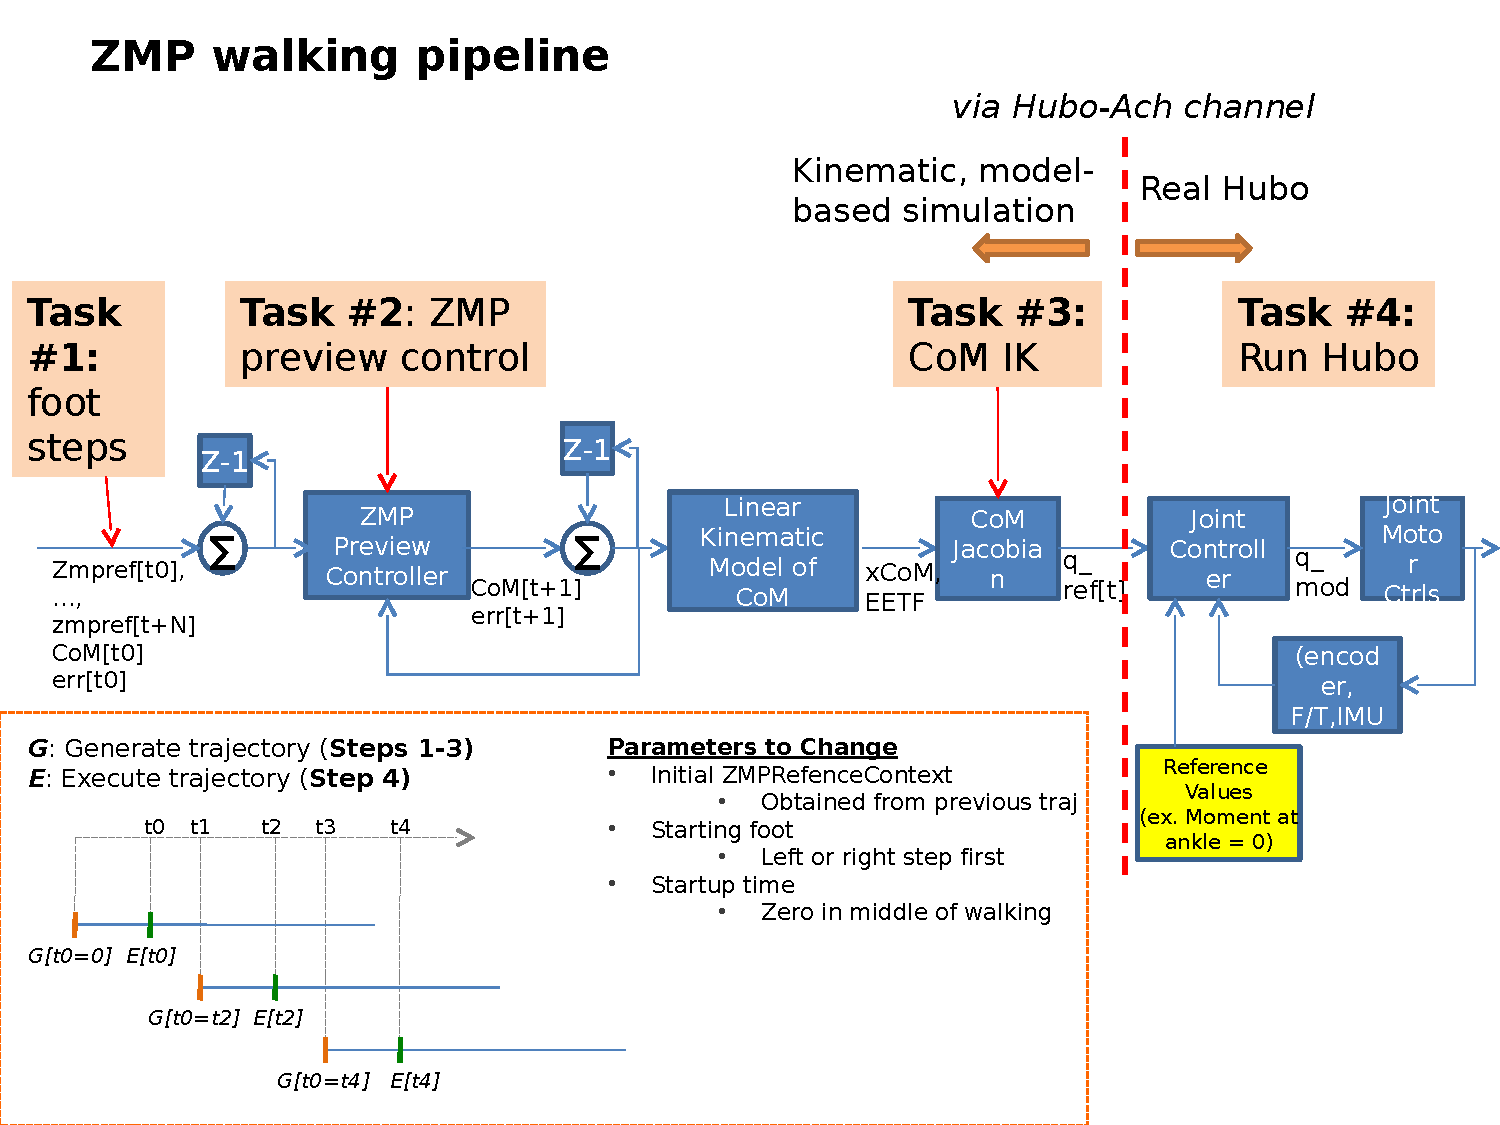
\includegraphics[width=\linewidth]{resources/zmp-walking-pipeline}
\end{itemize}

\section*{Apr 29 - May 5}
\subsection*{Status}
\begin{itemize}
\item Generated evaluation times for the zmpdemo code for different types and
number of footsteps.
\item Gave final presentation with Xinyan on teleoperation.
\end{itemize}

\section*{Apr 22-28}
\subsection*{Status}
\begin{itemize}
\item Sungmoon and I then planned out a schedule of small tasks to complete
achieve receding horizon online ZMP trajectory generation.
\item Evaluate generation time of trajectories for different types and number of
footsteps.
\item Achieve receding horizon using a button on the keyboard to walk in a straight
line.
\item Implement receding horizon online ZMP trajectory generation using
forward/backward and sidestep left/right using the keyboard.
\item Nishiwaki, Koichi, et al. "Online generation of humanoid walking motion based on
a fast generation method of motion pattern that follows desired zmp."
Intelligent Robots and Systems, 2002. IEEE/RSJ International Conference on. Vol.
3. IEEE, 2002.
\item The next task after completing this will be to start incorporating the footstep
planner and different walk types.
\end{itemize}
\subsection{Future Milestones}
\begin{itemize}
\item Incorporation of footstep planner and different walk types.
\end{itemize}

\section*{Apr 15-21}
\subsection*{Status}
\begin{itemize}
\item Set the motion computer up to have a static ip address.
\item Read through the hubomz code and commented some of it. Primarily I commented the
ZmpPreview.h file, which is the actual zmp controller. The CoM inverse
kinematics was a little hard to understand, but I understand enough to move
forward with the finite horizon.
\item I read through the Nishiwaki (2002) paper which presents online generation of 
zmp walking trajectories. I modified Sungmoon's ZMP-Walking diagram and added
the online receding-horizon method.
\item Created presentation for TePRA with Rowland.
\end{itemize}

\section*{Apr 8-14}
\subsection*{Status}
\begin{itemize}
\item Juan and I repaired Hubo's right hand pinky and middle fingers. The pinky
just need the set screw that hold the pulley on the motor shaft tightened. The
middle finger was the one previously broken and we just re-glued it with krazy
glue.
\item I wrote a simple hand program to open and close the fingers using the keyboard.
In doing so I discovered a bug and investigated the Hubo-ach code with Grey and
came up with some possible culprits. Grey later fixed it.
\url{https://github.com/pvieira3/hubo-misc/blob/master/test-code/src/hand.cpp}
\item Set up everything for National Robotics Week and conducted the teleportation
with the kids.
\end{itemize}

\section*{Apr 1-7}
\subsection*{Status}
\begin{itemize}
\item I helped Xinyan daemonize Liberty and cleaned up everything.
\url{https://github.com/pvieira3/Liberty-Daemon}
\item I updated the teleop-arms and teleop-legs code to accept arguments and make it
easier to understand
\url{https://github.com/pvieira3/hubo-misc/blob/master/test-code/src/teleop-arms.cpp}
\item I made a separate Collision\_Checker class. Currently, there's only a checker for
the arms, but a legs one will be added in the future.
\url{https://github.com/pvieira3/hubo-misc/blob/master/test-code/src/Collision\_Checker.cpp}
\url{https://github.com/pvieira3/hubo-misc/blob/master/test-code/include/Collision\_Checker.h}
\item I worked with Juan to get started tested grasping with the fingers. We
discovered the control daemon had some bugs related to the fingers because they
were never needed and therefore never tested and debugged. We notified Grey and
he fixed the bugs.
\item I thoroughly explained the impedance controller to Xinyan, which helped me
understand some details I was unaware of.
\item I updated the Fastrak class to accept the Fastrak or the Liberty tracker and
renamed it to Teleop.cpp
\url{https://github.com/pvieira3/hubo-misc/blob/master/test-code/src/Teleop.cpp}
\url{https://github.com/pvieira3/hubo-misc/blob/master/test-code/include/Teleop.h}
\item I fixed the compiler issues with Max's testIK.cpp code which he wrote to do a
unit test on the FK/IK for Hubo.
\end{itemize}

\section*{Feb 18-24}
\subsection*{Status}
\begin{itemize}
\item Xinyan and I got the Polhemus Liberty tracker fully working and tested. We
removed Fastrak completely and are now only using Liberty.
\item I added a simple self-collision avoidance function based on an ellipse-shaped
boundary. I added it to Hubo\_Control.cpp and ellipse parameters to
Hubo\_Control.h in my forked repo on the collision-avoidance branch.
\item I helped Andrew a bit to debug issues with hubo\_state and with moving the hand
to the location of the red object. He got that working! Videos are on his page.
\item Helped get Max started on writing a UnitTest for the FK and IK.
\item The working zmpdemo walking parameters for the video were:
\begin{itemize}
\item ./zmpdemo ../myhubo.kinbody.xml -w canned -z 0.06 -y 0.0885 -d 0.01 -s 0.5 -A -c
\item 8 -p 2 -X 0.038 -h 0.5 -l 0.08
\item -w: walk type "canned", meaning straight line
\item -z: foot vertical lift-off height of 0.06m
\item -y: half distance between feet of 0.0885m
\item -d: double-support time of 0.01s
\item -s: single-support time of 0.5s
\item -c: max number of step = 8
\item -p: initial time spent with zmp stationary = 2s
\item -l: max length of footstep = 0.08m
\item -X: forward distance from ankle to zmp = 0.04m
\item -A: use ach
\end{itemize}
\item Sungmoon and I tried tuning the walking parameters as well as tried adding
gradually reduced step size steps at the end of the walk. This helped a little
bit. Raising the COM z-position from 0.48m to 0.50m and changing the zmp
distance in front of the ankle from 0.04m to 0.038m helped.
\item Sungmoon and I wrote an impedance controller for the arm, using the torque
sensors in the wrist.
\item Code:
\url{https://github.com/pvieira3/hubo-misc/blob/master/test-code/src/impCtrl-arms.cpp}
\item Code: \url{https://github.com/pvieira3/hubo-misc/blob/master/test-code/include/impedanceController.h} 
\end{itemize}

\section*{Mar 11-17}
\subsection*{Status}
\begin{itemize}
\item Rowland and I went through Matt Zucker's walking code and learned how he
was spoofing input for the z-coordinate (height) of the feet in order to
construct a zmp trajectory in the y-direction, which was being fed into his ZMP
Preview controller, which spat out COM trajectory. This was then used with the
inverse kinematics to obtain full-body joint trajectories.
\item Rowland and I started adding code to get forward movement of the feet and body.
\item Rowland and I finished adding forward walking to the code and kinematic
visualization with Matt's help.
\item I helped Saul understand and re-factor the zmpdemo.cpp code.
\item I watched and learned from Matt about how we were going to break the code into
multiple objects.
\item I added the details for the runZMPPreview(), runCOMIK() and dumTraj() functions
in our zmpWalkingGenerator.
\item I helped out with the actual implementation of the code on Hubo and figuring out
how to control Hubo's balancing such that walking would be possible.
\item Code: \url{https://github.com/golems/hubomz}
\end{itemize}

\section*{Mar 4-10}
\subsection*{Status}
\begin{itemize}
\item Over the weekend Hubo's Right Hip Roll joint "broke" somehow. I took out
the control board and discovered that ground trace from the power socket to one
of the MOSFETs was burned out due to over-current. We swapped power, encoder and
limit switch cables with the Right Hip Yaw and turned on motor control with
Hubo-i and it worked fine. Therefore, there should be no issues mechanically,
and just a replacement of the board should fix the problem. The cause of the
failure is still not clear. We are aware that Hubo was designed with pretty much
no safety factors, so if somehow he was being commanded to stand, etc. for too
long without cooling down then an over-current may have occurred naturally. This
just means we need to be more conscious of Hubo's limits and how we test him.
\item Pushkar helped me install Dart/Grip again from source with a different install
method for fcl. This got most of the tabs and worlds working, but not all of
them. Still can't install from the apt repo for some reason.
\item Worked on porting our Inverse Kinematics code over to Ivan's WalkingTab.
\item I helped XinYan test his Polhemus Liberty daemon by using it to send Liberty
sensor data from XinYan's computer to Hubo using achd and controlling Hubo's
right arm via the sensor. It worked, but seemed a bit different than when using
Fastrak. Need to do more testing, and test with the left leg to figure out why
it's different.
\end{itemize}

\section*{Feb 25 - Mar 3}
\subsection*{Status}
\begin{itemize}
\item Ana and I added a function to the Hubo\_Tech library that calculates the
center of mass w.r.t. the neck, which is the world frame for the FK and IK.
Ana and I starting writing a balance daemon that uses the center of mass model
and the force/torque sensors in the ankles.
\item The Ethernet cable connected to PC2 was tripped over and the plastic socket was
snapped off the circuit board on Hubo. I got a new socket from James Steinberg
in Van Leer, desoldered the old ethernet socket on the Smart Power board and
soldered on a new one.
\item I spent a day working with Ivan to figure out how to control joints easily in
Dart.
\item I finally installed Dart/Grip after doing a clean install of Ubuntu 12.04 but
the worlds still wouldn't load.
\end{itemize}
\subsection*{Reflection}
\begin{itemize}
\item For walking a clear state machine idea has been formed, but we just need
to implement it.
\item For Dart/Grip I will talk to Pushkar, etc. on Monday to resolve the issues.
\end{itemize}

\section*{Feb 18-24}
\subsection*{Status}
\begin{itemize}
\item Andrew and I tested running a program on PC1 and sending the commands over
Ach to PC2 and while the daemons were running on PC2, but we are having issues.
We are doing something wrong with the communication.
\item I got the Polhemus Liberty working with PiTerm. I then wrote a simpler version
that got rid of all the GTK GUI stuff. I still need to parse the string of data
into an array and daemonize it.
\item XinYan and I tested the leg FK/IK and discovered that the problem was Grey's
ordering of the leg joints in control-daemon.h was different than that of
Rowland and me. The Hip Yaw and Hip Pitch were switched, so Grey changed them to
match our FK/IK.
\item I also discovered that because we had that miscommunication about the joint
ordering, the limits for the Hip Yaw and Pitch in our IK solution were swapped!
\item XinYan and I got Fastrak working with the legs. However, we discovered that the
leg IK doesn't handle the situation when the goal position is outside the
workspace properly, and returns -nan as the goal joint angle for the Hip Pitch,
Knee and Ankle Pitch. We are working on fixing this.
\item Andrew and I were able to read the state channel from the Vision PC, but not
write to the Ref channel.
\item I fixed the Leg IK code. It was returning -nan for joints 3, 4 and 5 (RHP, RKN
and RAP) when the goal was outside the workspace. I changed the square roots in
the calculations of the joint angles to be csqrt (complex sqrt) and changed the
radical to type 'double complex'. The norm between the goal position and the
solution positions wasn't being calculated with the correct goal position
because it was changed at the top of the function. The ordering of the limits
for the leg joints was wrong as well, because the hip pitch and hip yaw values
were switched.
\item I wrote a program to control the position and orientation of the feet using two
Fastrak sensors! It works really well, and has no issues when you move the
sensors outside the workspace of the feet.
\item Ana and I integrated her dart\_Lite library into the hubo-motion-rt library and
verified that it loads the URDF file in successfully.
\item I helped get XinYan set up with Liberty and he got it working on his own laptop
with Ubuntu via USB. He will continue to finish the writing of the read function
and daemon.
\item I took the neck off Hubo and tightened the loose screws so that if a camera is
temporarily mounted on the neck, any unnecessary looseness wouldn't be a
problem.
\item Hubo 4-Limb Teleoperation: Hubo's four limbs are being controlled using 4
different motion tracking sensors from the Polhemus Fastrak device. I have a
sensor taped to each foot and one in each hand. We are using the relative
translation of the sensors and the absolute orientations relative to the Fastrak
base station. These transformations are mapped to Hubo's hands and feet using
the inverse and forward kinematics of the arms and legs. Using an instantaneous
transformation to, for example, the Fastrak sensor in my left hand, we input
that transformation, or pose, into the inverse kinematics for Hubo's left arm to
determine the best joint angles solutions to produce that position and
orientation of the hand. The inverse kinematics generates eight possible
solutions, of which only a few could be possible, given joint limits and and
workspace considerations. If no solution contains six joint angles that are
within the joint limits, then the solution that gives a position closest to the
goal position is found by taking the norm of the vector between the goal
position and the position given a solution of joints that are scaled to comply
with the limits.
\item Code for teleop of the arms: \url{https://github.com/pvieira3/hubo-misc/blob/master/test-code/src/fastrak-arms.cpp}
\item Code for teleop of the legs: \url{https://github.com/pvieira3/hubo-misc/blob/master/test-code/src/fastrak-legs.cpp}
\end{itemize}


\section*{Feb 11-17}
\subsection*{Status}
\begin{itemize}
\item Writing code to test the leg IK and FK. Will use it to first squat, and
then balance on one leg.
\end{itemize}

\section*{Feb 04-10}
\subsection*{Status}
\begin{itemize}
\item Read papers on ZMP and Preview Control
\item Gave a presentation to the class with Eric Huang and Grey about locomotion,
which included static and dynamic walking, ZMP and Preview Control.
\item Continued updating the code for standing on one foot.
\item Fixed a bunch of mistakes in the Hubo Kinematics Tech Report and added to the
abstract.
\item Helped Grey run my squatting code to demo for ABC
\item Worked with Clayton to create a better side-by-side video of Hubo cutting a
rectangle in cardboard using Adobe Premiere.
\end{itemize}
\subsection*{Reflection}
\begin{itemize}
\item Need to make sure we export from Adobe Premiere as mp4 format.
\item Creating both 4:3 and 16:9 aspect ratio videos is useful for presentations and
watching videos, respectively.
\end{itemize}

\section*{Jan 28 - Feb 03}
\subsection*{Status}
\begin{itemize}
\item Added comments to the Hubo\_Tech header using Doxygen commenting style.
\item Started writing program to have Hubo stand on one leg using center of mass for
the feedback term
\end{itemize}
\subsection*{Reflection}
\begin{itemize}
\item Need to generalize code more as opposed to hard coding actions.
\end{itemize}


\section*{Jan 21-27}
\subsection*{Status}
\begin{itemize}
\item Rowland, Grey and I successfully cut out a 15x10cm square in
cardboard using Fastrak motion tracking for the right hand and for squatting.
\item Rowland and I finished writing the TePRA paper and submitted it.
\item Rowland and I also fixed the IK and FK code so that the teleoperation in
workspace works for 3-DOF.
\item Ana and I tested a simple version of center of mass calculation for the right
leg. When we moved the leg, the location of the center of mass moved in the
correct directions, but not with correct magnitudes. 
\item Hubo Cutting Rectangle in Cardboard: 01/25/2013. This is a video of Hubo cutting
a 15x10cm rectangle in cardboard, with two different camera angles, a main
closeup view of the cut, and a second, smaller view in the top-right corner of
the board, Hubo and the teleoperator in the background. We balanced him using
his ankle motors, which are velocity controlled using just a proportional term.
They are compliant with the moments about his ankles, but resistant against the
angle of his torso with respect to the vertical in order to keep him upright. He
has a Dremel strapped to his hand with a drill bit insert. We use the inverse
kinematics of the arm and a Polhemus Fastrak Motion Tracking device to move his
arm horizontally. By lowering the tracking device, Hubo also lowers by bending
at the knees. These two degrees of freedom allow Hubo to cut out the rectangle.
\end{itemize}

\subsection*{Reflection}
\begin{itemize}
\item The modeling of the center of mass is going a little slow, because the
URDF file is hard to interpret and doesn't seem accurate.
\end{itemize}


\section*{Jan 14-20}
\subsection*{Status}
\begin{itemize}
\item I was able to get Hubo to squat on Monday with just a bit of sway. The
sway is due to the fact that the ankles are not matching the speed of the hips,
which causes the torso to lean forward or backwards, so when Hubo stops moving
he has to rotate his ankles to return his torso to the vertical orientation.
This can be solved possibly by adjust the gains on the ankle pitch velocity.
\item Grey and I performed cardboard cutting with the Fastrak and the dremel. We
used the Drill IK that Rowland wrote and just varied the y-position in order to
create a smooth cut along a straight line. We were able to get Hubo to cut an
8-inch line in the cardboard, but then the wrist broke loose due to experience a
torque greater than its maximum allowable.
\item We also performed teleoperation of the dremel arm while using another sensor to control squating. We achieved this by using the dimensions of Hubo and some simple trigonometry.
\item I helped Andrew to get a webcam tracking a red piece of paper. Then, as the paper moved across the webcam's view, Hubo would move his arm in the same directions along the y-z plane. Andrew got this working using OpenCV and Boost for the vision and object tracking, and sockets in order to send the relative motions to Hubo's Linux computer. We need to adjust some of the transformations since Hubo's arm was not responding exactly as we expected.
\item I wrote a program to control both of Hubo's arms with the Fastrak sensors, as well as his waist with a third sensor. It is slightly different than the original one that Grey wrote, which didn't perform as hoped, possible due to the IK solutions and possibly due to there only being six DOF controlling six DOF, coupled with Hubo's limited worskpace. I will test my version on Monday, January 21st.
\item Hubo Squatting: 01/18/2013. This is a video of Hubo balancing and squatting. His ankles are velocity controlled using just a proportional term. They are compliant with the moments about his ankles, but resistant against the angle of his torso with respect to the vertical in order to stay upright. He squats by adjusting the velocity of his knee joints and then setting the hip and ankle joints to half the knee velocity.
\item Hubo Balancing \& Teleop (LEFT): 01/18/2013. This is a video of Hubo being controlled via teleoperation to balancing, squat and move his right arm. He balances using his ankles, which are velocity controlled using just a proportional term. They are compliant with the moments about his ankles, but resistant against the angle of his torso with respect to the vertical in order to stay upright. We use the inverse kinematics of the arm and move it horizontally using a Polhemus Fastrak Motion Tracking device. He squats by adjusting the velocity of his knee joints and then setting the hip and ankle joints to half the knee velocity.
\item Hubo Wall Cut (RIGHT): 01/18/2013. This is a video of Hubo cutting a line in cardboard. He balances using his ankles, which are velocity controlled using just a proportional term. They are compliant with the moments about his ankles, but resistant against the angle of his torso with respect to the vertical in order to stay upright. He has a dremel with a drill bit strapped to his hand. We use the inverse kinematics of the arm and move it horizontally using a Polhemus Fastrak Motion Tracking device.
\end{itemize}

\subsection*{Reflection}
\begin{itemize}
\item The balancing and squating work fine, but for anything more, we need the calculation of the center of mass. This way we won't have to rely on the IMU and we can just give a point of the floor for where to put Hubo's center of mass. This should make it possible to walk in a logical manner.
\item The webcam object tracking control of Hubo's arm exhibited some good response, but I definitely mixed up the IK for the drill and the hand and thus the transformations are wrong. This is an easy fix though.
\end{itemize}

\subsection*{Milestones}
\begin{itemize}
\item Get data for the wall cutting. We will get Fastrak data and Forward Kinematics data, and plot the two against each other.
\item Pick an object up with two hands using Fastrak.
\item Get the calculation of the center of mass and verify that it's correct
\end{itemize}

\section*{Jan 07-13}
\subsection*{Status}
\begin{itemize}
\item Finished writing the rough draft of the TePRA 2013 paper \href{https://thebrain.golems.org/svn/papers/2013/TePRA-13-hubo\_teleopTasks/}
{"Humanoid Robot Teleoperation for Dual-Arm Tasks with Power Tools"} with Rowland
O'Flaherty. This paper presents the implementation of inverse kinematics to
achieve teleoperation of a physical Hubo+ robot platform. Using a closed-form
kinematic solution and a basic feedback controller, teleoperation of simple
tasks is realized. The Hubo+ platform will be used to compete in the DARPA Robot
Challenge, which requires autonomous execution of various tasks; such as,
cutting through walls and moving rumble. Joint limits and singularities are
accounted for using the different cases in the kinematic solution; and a
decision method is implemented to determine how to position the end-effector
when the goal is outside the feasible workspace.
\item Achieved balancing with Grey. We did this by using velocity control
for the pitch and roll joints of the left and right ankles. We designed the
controller so that the ankles are compliant with the moments about the ankle
joints, but resistant against the waist IMU angle. These are both proportional
terms. We originally tried using position control with P, PD and PID type
controllers but found that oscillation would occur. The following is the code we
used.
\end{itemize}

\subsection*{Reflection}
\begin{itemize}
\item We had some trouble getting Hubo to bend at the knees and hips in
order to lower, but Grey had an idea to set the ankle velocity equal to the hip
velocity.
\end{itemize}

\subsection*{Milestones}
\begin{itemize}
\item Get Hubo to act like a spring, where if you press down on his
shoulders he'll lower, keeping his back vertical, and if you let off he'll rise
back up.
\item Cut through cardboard with the dremel by using the IK for the arm and
bending his legs in order to increase range of drilling motion.
\item Update the TePRA paper with results from dremel experimentation and
hopefully moving "rubble."
\end{itemize}

% -------------------------------------------------------------------------------------
% REFERENCES
% -------------------------------------------------------------------------------------
%\bibliography{}

% -------------------------------------------------------------------------------------
% END DOCUMENT
% -------------------------------------------------------------------------------------
\end{document}
